%% IEEE Access -- Supplementary Material
\documentclass[11pt]{article}
\usepackage[T1]{fontenc}
\usepackage{newtxtext}
\usepackage{newtxmath}
\usepackage[margin=1in]{geometry}
\usepackage{graphicx}
\usepackage{booktabs}
\usepackage{threeparttable}
\usepackage{longtable}
\usepackage{array}
\usepackage{float}
\usepackage{setspace}
\usepackage{caption}
\usepackage[numbers,sort&compress]{natbib}
\usepackage{hyperref}
\usepackage{titlesec}
\usepackage[nopatch=footnote]{microtype}
\setlength{\emergencystretch}{3em}
\captionsetup{font=small,labelfont=bf}
\hypersetup{hidelinks,
  pdftitle={DeepDTA-iBAM: Cross-Attention Interaction Mapping for Affinity Prediction, Ligand Retrieval, and Analog Generation (supplementary material)},
  pdfauthor={Kevin Song, John Zhang, Lei Ye, and Jianyi Zhang}}
\graphicspath{{../results/}}
\titleformat{\section}{\normalfont\large\bfseries}{\thesection}{1em}{}
\titleformat{\subsection}{\normalfont\normalsize\bfseries}{\thesubsection}{1em}{}
\renewcommand{\thesection}{S\arabic{section}}
\renewcommand{\thesubsection}{S\arabic{section}.\arabic{subsection}}
\renewcommand{\thefigure}{S\arabic{figure}}
\renewcommand{\thetable}{S\arabic{table}}
\newenvironment{smalltable}%
{\begin{table}[!htbp]\centering\begingroup\setlength{\tabcolsep}{3pt}\renewcommand{\arraystretch}{1.1}\footnotesize}%
{\endgroup\end{table}}

\begin{document}
\typeout{MANUSCRIPT_TEXT_WIDTH_PT=\the\textwidth}
\onehalfspacing

\begin{center}
{\Large\bfseries Supplementary Material\par}
\vspace{0.6\baselineskip}
{\normalsize for\par}
\vspace{0.4\baselineskip}
{\large\bfseries DeepDTA-iBAM: Cross-Attention Interaction Mapping for Affinity Prediction, Ligand Retrieval, and Analog Generation\par}
\vspace{0.9\baselineskip}
{\normalsize Kevin Song$^{1}$, John Zhang$^{1}$, Lei Ye$^{1}$, and Jianyi Zhang$^{1,*}$\par}
\vspace{0.5\baselineskip}
{\small $^{1}$Department of Biomedical Engineering, The University of Alabama at Birmingham,\\ Birmingham, Alabama, USA\par}
\vspace{0.3\baselineskip}
{\small $^{*}$Corresponding author: Jianyi Zhang; \href{mailto:jayzhang@uab.edu}{jayzhang@uab.edu}\par}
\end{center}

\vspace{1.0\baselineskip}

This supplementary information extends the main manuscript with uncertainty estimates, panel compositions, derivations, and compound-level outputs. These materials document where the reported conclusions are stable, where they remain sensitive to evaluation design, and how the underlying benchmark outputs were organized. All sections, subsections, figures, and tables use canonical supplementary numbering with the \texttt{S} prefix.

Four findings from the main text carry into this file and should be kept in view when reading it. First, atom-level contact metrics in the structural localization benchmark are saturated, because the atom contact base rate is 96.3 to 100\%. Atom contact AUROC is undefined in 4 of 5 complexes; the residue-level metrics remain valid and are analyzed in the main text by inverse-variance pooling. Second, the EGFR retrieval panel defined its positive class using a fingerprint similarity cutoff to the reference binders from which the anchors were drawn. The class-conditional similarity distributions are entirely disjoint, positives spanning 0.400 to 0.904 and decoys 0.054 to 0.233, so fingerprint baselines are not valid comparators on that panel, no similarity-matched subpanel can be constructed from these candidates, and the latent and affinity results are also conditional on this selection rule. Third, head-to-head comparisons between rankers scored on a shared candidate set require a paired test; marginal intervals reported in the tables below overlap in cases where the paired difference is nevertheless decisive. Fourth, the set of 100 diffusion analogs contains the dasatinib seed itself and 39 structures carrying implausible motifs, and its 100 canonically unique SMILES collapse to a single Bemis--Murcko generic framework; the audited set is reported in the main text.

The two assay-defined retrieval comparisons, the out-of-domain H1 panel and the in-domain EGFR panel with assay-defined actives and property-matched decoys, are reported in the main text; the construction of the latter is documented in Section~S7. Section~S2.1 documents the circular panel's composition in full, Section~S3.1 gives the label counts behind the saturation result, Section~S5 derives the power calculation quoted in the main text, and Section~S6 reports an audit of reporting practice in 25 published studies, so every diagnosis can be checked directly against the released data.

%% ------------------------------------------------------------------
\section{Additional Benchmark Context}
%% ------------------------------------------------------------------
The following benchmark material expands the evaluation on the custom random 90/5/5 KIBA split (termed standard in the main text) with uncertainty and scaffold-aware context, clarifying how stable the main benchmark estimates are and how they should be interpreted relative to more chemically stringent settings.

\subsection{Residual Diagnostics}
The main text reports pooled ranking performance while limiting
single-compound interpretation because of the width of the limits of agreement. Fig.~\ref{fig:residuals} shows a small overall mean bias
of $-0.010$, although residual medians vary modestly across the measured range.
Dispersion remains substantial: the 95\% limits of agreement span
$-0.895$ to $0.876$ KIBA units,
showing substantial individual prediction error despite the small mean bias.
These pooled diagnostics do not establish accuracy within individual target series.

\begin{figure}[!htbp]
\centering
\IfFileExists{../results/fig_residual_diagnostics.pdf}{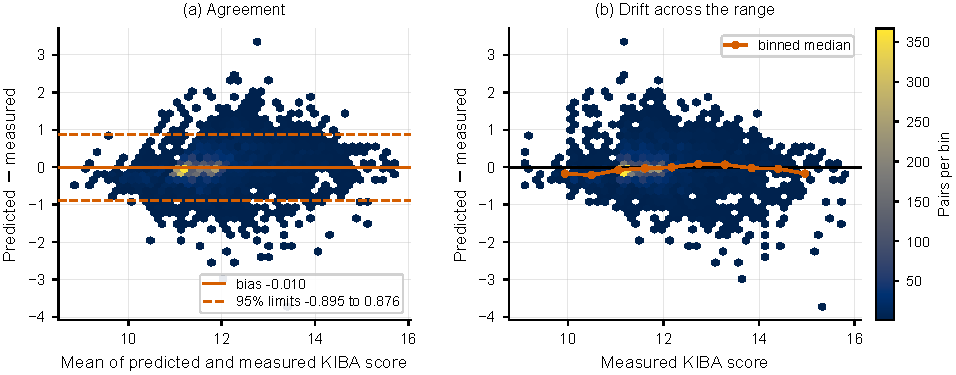
\includegraphics[width=0.98\linewidth]{../results/fig_residual_diagnostics.pdf}}{\fbox{Pending figure}}
\caption{\textbf{Residual diagnostics for the standard-split KIBA evaluation
($n = 5{,}913$ held-out pairs).} (a) Bland--Altman agreement between predicted
and measured KIBA score, with the mean bias and the 95\% limits of agreement.
(b) Residual against the measured value, with medians for bins containing at
least 20 observations among 12 equal-width bins. Both panels use hexagonal
binning, and the shared color scale gives the count per bin. The overall bias
is small relative to the dispersion, which limits single-compound use.}
\label{fig:residuals}
\end{figure}

\subsection{Bootstrap Uncertainty}
The bootstrap table below complements the primary benchmark values by showing local uncertainty around the reported point estimates. These intervals describe evaluation uncertainty for the saved checkpoint, but they should not be mistaken for between-study uncertainty because the literature benchmark rows were not rerun in a shared environment. Two concordance index values are computed from the same saved predictions using different conventions for ties. The main text reports 0.8625, from the released \texttt{analysis/analysis\_benchmark\_metrics.py}, which excludes pairs with equal measured values and counts pairs with equal predictions as half a concordance, consistent with the comparison methods. Table~\ref{tab:standard_bootstrap} reports 0.8621, the earlier in-house point estimate that scored prediction ties as zero, accompanied by a 600-resample bootstrap interval. The archived ablation summary differs for a separate reason: it averages three independently trained seeds rather than this single saved rerun.

\begin{smalltable}
\caption{\textbf{Bootstrap uncertainty for the single-checkpoint standard-split evaluation.}}
\label{tab:standard_bootstrap}
\IfFileExists{table_s_standard_eval_bootstrap.tex}{\begin{tabular}{lrrr}
\toprule
Metric & Estimate & 95\% CI lower & 95\% CI upper \\
\midrule
RMSE & 0.4517 & 0.4365 & 0.4672 \\
MAE & 0.2950 & 0.2869 & 0.3046 \\
Concordance & 0.8621 & 0.8556 & 0.8676 \\
Pearson $r$ & 0.8741 & 0.8634 & 0.8840 \\
$R^2$ & 0.7049 & 0.6795 & 0.7269 \\
\bottomrule
\end{tabular}
}{\fbox{Pending table}}
\par\vspace{3pt}
\begin{minipage}{\linewidth}\footnotesize\raggedright
Metrics were recomputed over 600 bootstrap resamples of the held-out prediction pairs ($n = 5{,}913$) to obtain nonparametric 95\% confidence intervals. RMSE and MAE are root-mean-square error and mean absolute error in KIBA units; CI denotes confidence interval; $r$ is Pearson correlation; $R^2$ is the coefficient of determination. These intervals quantify local evaluation uncertainty. The custom random KIBA split differs from published benchmark folds, so between-paper comparisons remain contextual.
\end{minipage}
\end{smalltable}

\subsection{Scaffold-Split Ablation Context}
The archived scaffold-split ablation summary evaluates model variants under a more chemically stringent split. Differences in mean concordance are modest relative to variability across three retraining seeds, limiting conclusions about the contribution of each component.

\begin{figure}[!htbp]
\centering
\IfFileExists{../results/fig_ablation_scaffold_summary.pdf}{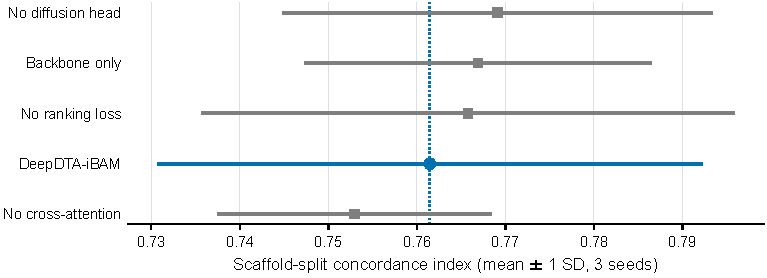
\includegraphics[width=0.98\linewidth]{../results/fig_ablation_scaffold_summary.pdf}}{\fbox{Pending figure}}
\caption{\textbf{Scaffold-split ablation summary from the archived three-seed aggregate results.} Markers give the mean scaffold-split concordance index across three retraining seeds and bars span one standard deviation, for the full model (blue circle, dotted reference line) and each ablated variant. A higher concordance index means better ranking agreement under chemistry shift. The means differ modestly relative to between-seed variability; these bars do not constitute a formal paired comparison. The no-diffusion-head and backbone-only variants have slightly higher means, and no-cross-attention the lowest. The main text reports a separate inference-time ablation of the fusion pathway.}
\label{fig:fig_ablation_scaffold_summary}
\end{figure}

%% ------------------------------------------------------------------
\section{Retrieval Analyses}
%% ------------------------------------------------------------------
These materials document the composition of the circular EGFR panel and its full metric set. ECFP rows in those tables are leakage diagnostics rather than comparators, and the remaining results are conditional on the same selection rule. H1 replicate values are available in \path{results/h1_drug_fishing_replicate_metrics.csv}.

\subsection{EGFR Panel Composition and the Fingerprint-Circularity Diagnosis}
The EGFR family was assembled from ChEMBL target CHEMBL203 by filtering exact-binding records to molecules with pChEMBL $\geq$ 7.0 and Morgan/ECFP Tanimoto similarity $\geq$ 0.40 to gefitinib (CHEMBL939) or erlotinib (CHEMBL553). All 347 retained molecules satisfy the similarity criterion by construction, with an observed minimum of exactly 0.4000, a mean of 0.5011, and a maximum of 1.0000. The 6 interpolation anchors were then drawn from within this same family, and the 2,000 ZINC decoys were sampled with no similarity constraint.

A nearest-anchor ECFP ranker evaluated on this panel is thus scored on the criterion that defined the positive class. The observed consequence is perfect separation with a degenerate bootstrap interval (AUROC $=$ 1.000 with 95\% CI [1.000, 1.000], AUPRC $=$ 1.000, and BEDROC20 $=$ 1.000), consistent with selection-rule circularity. Model-derived rankings remain mutually comparable on this selected panel, but their absolute performance is conditioned on its similarity-based composition. Section~S7 documents the assay-defined replacement panel.

\subsection{Expanded EGFR Retrieval Outputs}
The following tables provide the full retrieval metric set, including the exploratory combined score, together with the top exploratory ZINC candidates. The saved circular panel used 6 anchors, 341 holdouts, 2,000 local ZINC decoys, and a 500-resample candidate-set bootstrap.

\begin{smalltable}
\caption{\textbf{Full EGFR retrieval benchmark, including the exploratory combined path-plus-affinity score.}}
\label{tab:egfr_full_metrics}
\IfFileExists{table_s_egfr_retrieval_metrics_full.tex}{\resizebox{0.97\linewidth}{!}{\begin{tabular}{lrrrrrrr}
\toprule
Method & AUROC & AUPRC & BEDROC20 & EF at 1\% & EF at 5\% & Recovery at 5\% & Recovery at 10\% \\
\midrule
Interpolation path & 0.8152 & 0.5378 & 0.6774 & 6.8651 & 5.5270 & 0.2786 & 0.3812 \\
Latent nearest anchor & 0.7958 & 0.5092 & 0.6522 & 6.8651 & 5.2943 & 0.2669 & 0.3519 \\
Predicted affinity & 0.9495 & 0.9250 & 0.9757 & 6.8651 & 6.8651 & 0.3460 & 0.6774 \\
Nearest-anchor ECFP & 1.0000 & 1.0000 & 1.0000 & 6.8651 & 6.8651 & 0.3460 & 0.6891 \\
Anchor-centroid ECFP & 1.0000 & 1.0000 & 1.0000 & 6.8651 & 6.8651 & 0.3460 & 0.6891 \\
Combined (exploratory) & 0.9484 & 0.8574 & 0.9337 & 6.8651 & 6.8651 & 0.3460 & 0.6540 \\
\bottomrule
\end{tabular}
}}{\fbox{Pending table}}
\par\vspace{3pt}
\begin{minipage}{\linewidth}\footnotesize\raggedright
The circular panel contains 341 holdouts and 2,000 decoys (positive fraction, 0.146). AUROC and AUPRC denote areas under the receiver operating characteristic and precision-recall curves; BEDROC20 is Boltzmann-enhanced discrimination of ROC with $\alpha = 20$. EF denotes enrichment factor; recovery is the fraction of holdouts retrieved at the stated ranked fraction. The combined score reuses model-derived information in latent geometry and affinity scoring and is included because it ranked the exploratory ZINC hits. ECFP denotes extended-connectivity fingerprint; its rows are leakage diagnostics, not comparators.
\end{minipage}
\end{smalltable}

\begin{smalltable}
\caption{\textbf{Top 10 exploratory ZINC candidates ranked by the combined interpolation and affinity score.}}
\label{tab:egfr_top_hits}
\IfFileExists{table_s_top_egfr_retrieval_hits.tex}{\resizebox{\linewidth}{!}{\input{table_s_top_egfr_retrieval_hits.tex}}}{\fbox{Pending table}}
\vspace{3pt}
\begin{minipage}{\linewidth}\footnotesize
Predicted EGFR affinity is in KIBA units; path distance is measured in the model's latent space. Tanimoto denotes nearest-anchor ECFP similarity. QED is quantitative estimate of drug-likeness (higher is more favorable); SA is synthetic accessibility score (lower indicates easier synthesis). Lipinski and alert-free columns report pass status (1, yes; 0, no). Full SMILES strings are retained in the CSV artifact. These entries are exploratory follow-up candidates, not experimentally validated EGFR actives.
\end{minipage}
\end{smalltable}

%% ------------------------------------------------------------------
\section{Interpretability Outputs}
%% ------------------------------------------------------------------
The per-complex table below resolves the heterogeneity behind the structural-localization summary and makes the base-rate degeneracy directly inspectable.

\subsection{Contact Base Rates Underlying the Degeneracy Diagnosis}
Table~\ref{tab:base_rates} reports the label composition for each complex. Residue-level label vectors contain both classes (5.7--9.5\% positives), whereas atom-level label vectors are single-class in 4 of 5 complexes and contain exactly one negative in the fifth. Atom contact AUROC is therefore undefined in 4 of 5 complexes, and atom top-$k$ overlap, where $k$ is the number of true contacts, has a base-rate expectation of 0.993, against which the observed 0.992 represents an enrichment of 1.00$\times$.

\begin{smalltable}
\caption{\textbf{Label composition of the structural-localization benchmark.}}
\label{tab:base_rates}
\begin{tabular}{llrrrrrr}
\toprule
PDB & Protein & Residues & Contact res. & Res. rate & Atoms & Contact atoms & Atom rate \\
\midrule
1KE6 & CDK2   & 280 & 16 & 0.057 & 27 & 26 & 0.963 \\
2HYY & ABL1   & 263 & 25 & 0.095 & 37 & 37 & 1.000 \\
4RJ3 & CDK2   & 287 & 19 & 0.066 & 29 & 29 & 1.000 \\
4WKQ & EGFR   & 296 & 18 & 0.061 & 31 & 31 & 1.000 \\
6YOJ & FAK1   & 259 & 22 & 0.085 & 34 & 34 & 1.000 \\
\bottomrule
\end{tabular}
\par\vspace{3pt}
\begin{minipage}{\linewidth}\footnotesize\raggedright
For each complex, the number of residues and ligand heavy atoms is reported alongside the number and fraction annotated as crystallographic contacts at a 4.5~\AA{} heavy-atom cutoff. The atom-level contact fraction reaches 1.000 in 4 of 5 complexes, which renders atom contact AUROC undefined and saturates atom top-$k$ overlap.
\end{minipage}
\end{smalltable}

Table~\ref{tab:interpretability_per_complex} gives the per-complex localization scores
and perturbation results underlying the main-text summaries.

\begin{smalltable}
\caption{\textbf{Per-complex structural localization benchmark across 5 kinase co-crystal complexes.}}
\label{tab:interpretability_per_complex}
\IfFileExists{table_s_interpretability_per_complex.tex}{\resizebox{0.97\linewidth}{!}{\begin{tabular}{lllrrrrrr}
\toprule
PDB & Protein & Ligand & Residue AUROC & Atom AUROC & Residue top-$k$ & Atom top-$k$ & Residue mask & Atom mask \\
\midrule
1KE6 & CDK2 & LS2 & 0.6042 & 0.2692 & 0.0625 & 0.9615 & -0.0882 & 0.5457 \\
2HYY & ABL1 & STI & 0.7092 & NA & 0.2000 & 1.0000 & -0.0065 & -0.1940 \\
4RJ3 & CDK2   & 3QS & 0.7025 & NA & 0.1053 & 1.0000 & 0.0829 & -1.5489 \\
4WKQ & EGFR & IRE & 0.4243 & NA & 0.0556 & 1.0000 & 0.3978 & 1.1355 \\
6YOJ & FAK1 & P4N & 0.4860 & NA & 0.1364 & 1.0000 & -0.9607 & -0.3156 \\
\bottomrule
\end{tabular}
}}{\fbox{Pending table}}
\par\vspace{3pt}
\begin{minipage}{\linewidth}\footnotesize\raggedright
Each row reports residue-contact and atom-contact AUROC, top-$k$ overlap with $k$ equal to the number of true contacts, and perturbation signals for one protein--ligand pair. NA indicates undefined atom-contact AUROC for single-class labels; see Table~\ref{tab:base_rates}. Masking signals are differences in predicted-affinity reduction (KIBA units) between masking the top 10 tokens and masking 10 randomly selected tokens. Positive values favor the attention-selected set. The random control used one draw per complex, so uncertainty across random draws was not estimated.
Atom-contact labels were mapped from PDB order to the cached graph order by
enumerating all element- and bond-preserving mappings. All mappings give the
same contact vector for each complex. A targeted CPU rerun corrects the 1KE6
atom AUROC to 0.2692; the other atom AUROCs remain undefined and all atom
overlaps are unchanged. Residue metrics and masking results retain their
archived values. The audit is released as
\path{analysis/revalidate_atom_contacts.py}.
\end{minipage}
\end{smalltable}

%% ------------------------------------------------------------------
\section{Local Design Outputs}
%% ------------------------------------------------------------------
The remaining local-design materials provide compound-level context for the EGFR-conditioned analog-proposal benchmark. These outputs remain model-internal; the rule-based chemistry filters reported here are triage cues, not orthogonal validation of potency or developability.

\subsection{Structural Audit of the Generated Set}
The main text summarizes the audit of the 100 released diffusion analogs; Table~\ref{tab:generated_audit_s} gives it in full. The seed row is dasatinib itself, recovered at Tanimoto 1.000 and counted among the generated analogs. Structural alerts identify motifs excluded by the audit despite passing RDKit sanitization; molecules may carry more than one, and the final column gives how many of each class were nonetheless passed as alert-free by the PAINS/BRENK filter used in the original pipeline. Generic frameworks are Bemis--Murcko scaffolds with atom types and bond orders erased: the set collapses to one, so canonical-SMILES uniqueness does not measure scaffold diversity here.

\begin{smalltable}
\caption{\textbf{Structural audit of the 100 released diffusion analogs.}}
\label{tab:generated_audit_s}
\IfFileExists{table_generated_audit.tex}{\begin{tabular}{lrrrr}
\toprule
Stage & Molecules & Unique SMILES & Murcko scaffolds & Generic frameworks \\
\midrule
As released & 100 & 100 & 98 & 1 \\
Seed removed & 99 & 99 & 97 & 1 \\
Alert-filtered & 60 & 60 & 59 & 1 \\
\midrule
\multicolumn{3}{l}{\textit{Structural alerts removed (molecules may carry more than one)}} & \multicolumn{2}{r}{\textit{Passed PAINS/BRENK}} \\
\quad Peroxide O--O & 11 & & \multicolumn{2}{r}{0} \\
\quad Low-valent P & 4 & & \multicolumn{2}{r}{0} \\
\quad Ring hydrazine N--N & 17 & & \multicolumn{2}{r}{7} \\
\quad Ring hydroxylamine N--O & 18 & & \multicolumn{2}{r}{7} \\
\quad Any alert & 39 & & \multicolumn{2}{r}{13} \\
\bottomrule
\end{tabular}
}{\fbox{Pending table}}
\par\vspace{3pt}
\begin{minipage}{\linewidth}\footnotesize\raggedright
The upper block follows the set through the audit, from the released output, through removal of the dasatinib seed, to the 60 analogs surviving the structural-alert filter, counting distinct canonical SMILES, distinct Bemis--Murcko scaffolds and distinct generic frameworks at each stage. Canonical-SMILES and scaffold counts track the set size while the generic-framework count stays at one. The lower block breaks the removed molecules down by alert class, with the number of each class that the original PAINS/BRENK filter had nonetheless passed as alert-free.
\end{minipage}
\end{smalltable}

\subsection{Ranked Diffusion Analog Table}
SMILES and properties for all 60 analogs surviving the audit are in the released file \path{results/generated_egfr_analogs_audited.csv}.
Table~\ref{tab:diffusion_gallery} prioritizes chemical screening flags and QED.
The structure figure in the main text ranks this same pool by predicted KIBA
score alone, so the two selections serve different purposes.

\begin{smalltable}
\caption{\textbf{Top 10 diffusion analogs ranked by chemical filters and drug-likeness.}}
\label{tab:diffusion_gallery}
\IfFileExists{table_generated_top10.tex}{\resizebox{0.97\linewidth}{!}{\begin{tabular}{rlrrrrrcc}
\toprule
\# & Murcko framework (rings) & MW (Da) & cLogP & QED & SA & Tanimoto & Lip. & Alert-free \\
\midrule
1 & 4 rings (3 aromatic) & 445.6 & 3.96 & 0.550 & 3.74 & 0.123 & yes & yes \\
2 & 4 rings (3 aromatic) & 444.6 & 4.31 & 0.542 & 4.22 & 0.150 & yes & yes \\
3 & 4 rings (3 aromatic) & 444.6 & 4.36 & 0.540 & 3.34 & 0.140 & yes & yes \\
4 & 4 rings (3 aromatic) & 444.6 & 4.49 & 0.537 & 4.12 & 0.149 & yes & yes \\
5 & 4 rings (2 aromatic) & 452.6 & 1.53 & 0.523 & 4.10 & 0.157 & yes & yes \\
6 & 4 rings (3 aromatic) & 444.6 & 4.74 & 0.468 & 4.24 & 0.134 & yes & yes \\
7 & 4 rings (3 aromatic) & 445.6 & 4.94 & 0.457 & 4.04 & 0.127 & yes & yes \\
8 & 4 rings (3 aromatic) & 444.6 & 4.30 & 0.508 & 3.08 & 0.223 & yes & no \\
9 & 4 rings (3 aromatic) & 444.6 & 3.81 & 0.461 & 4.15 & 0.161 & yes & no \\
10 & 4 rings (3 aromatic) & 450.5 & 4.30 & 0.440 & 4.11 & 0.158 & yes & no \\
\bottomrule
\end{tabular}
}}{\fbox{Pending table}}
\par\vspace{3pt}
\begin{minipage}{\linewidth}\footnotesize\raggedright
Drawn from the 60 molecules surviving removal of the dasatinib seed and of the 39 structures carrying peroxide, low-valent phosphorus, or cyclic hydrazine and hydroxylamine motifs. Rows are ordered by Lipinski pass status, alert-free status, descending QED, ascending synthetic accessibility, and descending predicted EGFR affinity. All entries have four rings and share one Bemis--Murcko generic framework with dasatinib; aromatic ring counts can differ. MW is molecular weight in Da; cLogP is calculated octanol--water partition coefficient on a logarithmic scale. QED is quantitative estimate of drug-likeness; SA is synthetic accessibility score. Lip. denotes Lipinski pass status, and alert-free denotes passing the original PAINS/BRENK filter. Tanimoto is similarity to the dasatinib starting structure. These are model-internal follow-up candidates, not validated optimization outcomes.
\end{minipage}
\end{smalltable}

%% ------------------------------------------------------------------
\section{Power Calculation for the Structural-Localization Panel}
%% ------------------------------------------------------------------
The main text gives a conditional estimate of 18 to 21 co-crystal complexes to distinguish a residue contact AUROC of 0.585 from chance at 80\% power. This section gives the derivation and its assumptions. The calculation is implemented in \texttt{analysis\_power.py}.

\subsection{Design and Variance Components}
Complexes are the unit of replication. The five complexes represent four targets, including two CDK2 complexes, which limits target-level independence. Each complex $j$ supplies one residue contact AUROC $A_j$ estimated from its own 250 to 300 residues, so $A_j$ carries a within-complex sampling variance $s_j^2$ on top of a between-complex variance $\tau^2$. The within-complex variance is the analytic Hanley--McNeil quantity~\cite{hanley1982auroc},
\[
s_j^2 = \frac{A_j(1 - A_j) + (n^{+}_j - 1)(Q_1 - A_j^2) + (n^{-}_j - 1)(Q_2 - A_j^2)}{n^{+}_j n^{-}_j},
\]
with $Q_1 = A_j / (2 - A_j)$ and $Q_2 = 2A_j^2 / (1 + A_j)$, and $n^{+}_j$, $n^{-}_j$ the contact and non-contact residue counts. The between-complex variance is the DerSimonian--Laird estimator~\cite{dersimonian1986meta} applied to the same five complexes. On the observed panel these evaluate to
\[
\bar{s}^2 = 0.00455 \quad (\bar{s} = 0.067), \qquad \tau^2 = 0.01284 \quad (\tau = 0.113),
\]
so between-complex heterogeneity contributes roughly three times the variance that within-complex sampling error does. This is the quantitative form of the $I^2 = 74\%$ reported in the main text, and it is why adding residues to existing complexes cannot substitute for adding complexes.

\subsection{Required Panel Size}
Assuming independent complexes, a random-effects pooled estimate over $k$ complexes has
\[
\mathrm{Var}(\hat{A}_{\text{pooled}}) \approx \frac{\tau^2 + \bar{s}^2}{k} = \frac{0.01739}{k},
\]
so testing $H_0: A = 0.5$ against $A_1 = 0.585$ at two-sided $\alpha$ with power $1 - \beta$ requires
\[
k \;\geq\; \frac{(z_{1 - \alpha/2} + z_{1 - \beta})^2 (\tau^2 + \bar{s}^2)}{(A_1 - 0.5)^2}
 = \frac{(1.960 + 0.842)^2 \times 0.01739}{0.085^2} = 18.9,
\]
that is 19 complexes. Substituting the empirical complex-level variance (0.01631, without separating variance components) gives 18. Repeating the calculation with a one-sample $t$ test and power computed from the noncentral $t$ distribution gives 20 to 21. The resulting estimate is \textbf{18 to 21 complexes}. This range reflects the variance estimate and small-sample approximation; it does not include uncertainty in the assumed effect or variance components, which were estimated from only five complexes. Table~\ref{tab:power} gives the full curve.

The estimated power of the 5-complex panel under these assumptions is 0.30 under the normal approximation and 0.20 under the $t$ calculation. Thus, a nonsignificant result would be likely even if the assumed effect were present; these conditional calculations do not establish whether that effect is real.

\begin{smalltable}
\caption{\textbf{Statistical power by number of protein--ligand complexes.}}
\label{tab:power}
\IfFileExists{table_power.tex}{\begin{tabular}{rcccc}
\toprule
Complexes $k$ & SE of pooled AUROC & 95\% CI half-width & Power (normal) & Power ($t$) \\
\midrule
5 & 0.0590 & 0.1156 & 0.30 & 0.20 \\
10 & 0.0417 & 0.0817 & 0.53 & 0.44 \\
15 & 0.0340 & 0.0667 & 0.70 & 0.64 \\
20 & 0.0295 & 0.0578 & 0.82 & 0.78 \\
25 & 0.0264 & 0.0517 & 0.90 & 0.87 \\
30 & 0.0241 & 0.0472 & 0.94 & 0.93 \\
40 & 0.0208 & 0.0409 & 0.98 & 0.98 \\
50 & 0.0186 & 0.0365 & 1.00 & 0.99 \\
\midrule
\multicolumn{5}{l}{Variance components from the observed panel: $\tau^2 = 0.01284$, $\bar{s}^2 = 0.00455$} \\
\multicolumn{5}{l}{Estimated for 80\% power at $\alpha = 0.05$: $k = 18$ to 21 complexes} \\
\bottomrule
\end{tabular}
}{\fbox{Pending table}}
\par\vspace{3pt}
\begin{minipage}{\linewidth}\footnotesize\raggedright
Standard errors and power are conditional on variance components estimated from the observed 5-complex panel, $\tau^2 = 0.01284$ and $\bar{s}^2 = 0.00455$, and a target residue contact AUROC of 0.585 against chance at two-sided $\alpha = 0.05$. CI half-widths use the normal approximation. The normal power column uses the large-sample approximation; the $t$ column uses a one-sample $t$ test and the noncentral $t$ distribution. Neither calculation incorporates uncertainty in the assumed effect or variance components.
\end{minipage}
\end{smalltable}

%% ------------------------------------------------------------------
\section{Audit of Reporting Practice in the Published Literature}
%% ------------------------------------------------------------------
The reporting checks proposed in the main text are only worth proposing if they are not already standard. To test that, we audited 25 published drug--target affinity and compound--protein interaction studies for whether they apply them. The audit is implemented in \texttt{analysis\_literature\_audit.py} and its verdicts are released in \texttt{literature\_audit.csv}.

\subsection{Scope and Criteria}
Papers were drawn from Europe PMC and restricted to open-access full texts, so that every verdict can be checked by a reader against the same source we read. The sample spans 2018 to 2026 and mixes the canonical architectures (DeepDTA, DeepAffinity, MolTrans, MGraphDTA) with recent work through 2026. It is a convenience sample of the open-access literature rather than a systematic review, and it is not a random draw from all published models; papers behind subscription paywalls, including several widely cited ones, could not be included on the same terms and were excluded rather than assessed from their abstracts.

Each paper was read for four questions. Does it validate attention or importance scores against annotated binding-site or contact residues, in any form, including a purely visual case study? If so, is that validation quantitative, meaning it reports an overlap, enrichment, accuracy, intersection-over-union or AUROC number, rather than a picture with residues named in the caption? If quantitative, does the paper anywhere report the positive-class base rate, the fraction of residues that are pocket or contact residues, alongside the metric? And separately, does it define a positive or active set using a chemical similarity threshold or analog series while also scoring a fingerprint or similarity baseline on that same set? A paper that computes a base rate internally but does not print it is recorded as not reporting it, because the check we propose is a reporting practice rather than a computation.

\subsection{Result}
Sixteen of the 25 papers validate attention against annotated residues. Five of those 16 do so only visually, showing a heatmap or naming agreeing residues in a caption without any metric, which leaves nothing to check a base rate against. Eleven report a quantitative figure, and \textbf{3 of those 11 report the positive-class base rate beside it}. The remaining 8 report an enrichment, overlap, or accuracy number with no statement of what fraction of residues were positives, which is the condition under which base-rate saturation is invisible. The three exceptions (GGAP-CPI, CDPN, and LiBRe) show that the practice is achievable and is occasionally followed; two of the three are recent studies whose explicit purpose was benchmark quality.

The second criterion returned nothing. \textbf{None of the 25 papers scored a similarity baseline on a similarity-defined positive set}, so selection-rule circularity was not observed anywhere in this sample. The reason is structural rather than reassuring: most drug--target affinity papers do not build target-family retrieval panels at all, and those in this sample that ran virtual screening evaluations drew their actives from annotation databases such as DUD-E and LIT-PCBA rather than from a similarity cutoff. We therefore make no claim about how often selection-rule circularity occurs in published work. Eight of the eleven quantitative studies omit the base rate needed to assess saturation; the audit does not establish that their metrics were saturated. Selection-rule circularity was diagnosed in our own panel, and its prevalence in published work remains unknown.

\begin{smalltable}
\caption{\textbf{Audit of 25 published drug--target affinity and compound--protein interaction studies.}}
\label{tab:literature_audit}
\IfFileExists{table_literature_audit.tex}{\begin{tabular}{llrccc}
\toprule
Model / study & Venue & Year & Residue claim & Quantitative & Base rate \\
\midrule
DeepDTA & Bioinformatics & 2018 & no & -- & -- \\
DeepAffinity & Bioinformatics & 2019 & yes & yes & no \\
MolTrans & Bioinformatics & 2021 & yes & no & -- \\
MGraphDTA & Chem Sci & 2022 & yes & yes & no \\
AttentionSiteDTI & Brief Bioinform & 2022 & yes & no & -- \\
PIGNet & Chem Sci & 2022 & no & -- & -- \\
GraphATT-DTA & Biomedicines & 2023 & yes & no & -- \\
PocketDTA & J Cheminform & 2024 & yes & no & -- \\
CASTER-DTA & Brief Bioinform & 2025 & yes & yes & no \\
MIF-DTI & Brief Bioinform & 2025 & no & -- & -- \\
GGAP-CPI & J Chem Inf Model & 2025 & yes & yes & yes \\
CDPN & J Chem Inf Model & 2025 & yes & yes & yes \\
GPS-DTI & BMC Biol & 2025 & yes & yes & no \\
GenSPARC & Commun Chem & 2025 & yes & yes & no \\
HMM-DTA & J Cheminform & 2026 & no & -- & -- \\
ChemGLaM & J Cheminform & 2026 & yes & yes & no \\
DCI-SiteDTA & BMC Bioinformatics & 2026 & yes & yes & no \\
DTAP & Brief Bioinform & 2026 & yes & no & -- \\
TSEDTA & Bioinformatics & 2026 & yes & yes & no \\
DCGAT-DTI & Bioinform Adv & 2026 & no & -- & -- \\
TriDTI & Brief Bioinform & 2026 & no & -- & -- \\
MMCA & PLoS One & 2026 & no & -- & -- \\
Dual-encoder fusion & BMC Bioinformatics & 2026 & no & -- & -- \\
LiBRe & J Chem Inf Model & 2026 & yes & yes & yes \\
PhenoModel & Acta Pharm Sin B & 2026 & no & -- & -- \\
\midrule
\multicolumn{6}{l}{16 of 25 validate attention against annotated residues; 11 of those do so quantitatively} \\
\multicolumn{6}{l}{Of the 11 quantitative evaluations, 3 report the positive-class base rate and 8 do not} \\
\multicolumn{6}{l}{0 of 25 score a similarity baseline on a similarity-defined positive set} \\
\bottomrule
\end{tabular}
}{\fbox{Pending table}}
\par\vspace{3pt}
\begin{minipage}{\linewidth}\footnotesize\raggedright
\textit{Residue claim} is whether the paper validates attention or importance against annotated binding-site or contact residues in any form. \textit{Quantitative} distinguishes a reported metric from a visual case study. \textit{Base rate} is whether the fraction of residues that are pocket or contact residues is reported alongside that metric, and is not applicable where the validation is purely visual. All entries are open-access full texts, listed with their PMC identifiers in the released CSV so that each verdict can be checked.
\end{minipage}
\end{smalltable}

%% ------------------------------------------------------------------
\section{Construction of the In-Domain, Assay-Defined EGFR Panel}
%% ------------------------------------------------------------------
The main text reports an in-domain retrieval comparison that replaces the circular EGFR panel. This section documents how it was built, including one route that failed, because the failure is instructive about why property-matched decoys are hard to produce from a general-purpose compound library.

\subsection{Why the Decoys Are Not Drawn From a General-Purpose Library}
The saved exploratory EGFR candidate file contains 6,060 unique molecule IDs
and SMILES, each with pChEMBL $\geq$ 7.0 and a recorded measurement type of
$K_i$, IC$_{50}$, or $K_d$. This file and the consolidation cache are distinct
artifacts. The latter contains 5,976 potent molecule IDs, which consolidate to
5,942 parent IDs. All 5,976 are present in the exploratory file, together with
84 additional molecules: 73 are absent from the consolidation cache and 11
have only subthreshold potency in that cache. These counts explain the
numerical discrepancy; the historical query or database-version cause of the
different records cannot be established from the retained files.

Recomputing descriptors from the saved SMILES gives mean molecular weight
506.0\,Da and cLogP 4.77 for the 6,060 candidates, versus 253.6\,Da and 0.01 for
the 60,000-compound ZINC pool. The pool spans 199.2 to 438.3\,Da. Only 8
candidates fall within all six marginal descriptor ranges for molecular weight, cLogP,
hydrogen-bond donors and acceptors, rotatable bonds, and formal charge. This
range check does not establish that adequate matched neighbors exist. The
saved matching output contains one active and ten decoys, but its exact
historical matching criteria could not be reconstructed. These property
differences support using the DUD-E EGFR panel for the reported comparison;
the balance of that panel is quantified below. The reproducible audit is
released as \path{analysis/revalidate_egfr_curation.py}.

\subsection{The Panel Used}
DUD-E's EGFR target supplies actives defined by ChEMBL activity with decoys property-matched to them by construction~\cite{mysinger2012dude}. From its 542 actives and 35,050 decoys we sampled 300 and 3,000, respectively, under a fixed seed. Property balance between the classes, expressed as a standardized mean difference, is 0.06 for molecular weight, $-0.06$ for hydrogen-bond donors, 0.10 for rotatable bonds, 0.76 for hydrogen-bond acceptors, 0.88 for cLogP, and $-0.91$ for net formal charge. The first three are well matched; the last three retain substantial imbalance.

The class-conditional similarity diagnostic uses the maximum ECFP Tanimoto similarity to gefitinib or erlotinib, as for the circular panel. Here the supports \emph{overlap}: actives span 0.058 to 1.000 and decoys span 0.021 to 0.214, and the shared region contains 97 of the 300 actives and 2,950 of the 3,000 decoys. This overlap permits construction of a similarity-matched subpanel, although it does not establish an unbiased benchmark. The retrieval fingerprint baseline uses a separate definition: nearest-active similarity to all 300 panel actives, with each active excluded from its own reference set.

\subsection{What This Panel Still Does Not Settle}
DUD-E selects decoys that are topologically dissimilar to its actives. This does not define the positive class by similarity, but it can favor fingerprint methods. Published critiques show that models can perform well on such benchmarks by exploiting dataset biases~\cite{chen2019hiddenbias,wallach2018memorization}. The 0.153 AUROC gap between the fingerprint baseline and the model may therefore overstate the difference on a panel without topological decoy selection. Evaluating that difference requires an independent panel with experimentally supported inactive compounds, such as a suitable target-specific subset of LIT-PCBA~\cite{trannguyen2020litpcba}, and remains open.

\bibliographystyle{IEEEtran}
\bibliography{references}

\end{document}
